\documentclass[aspectratio=169]{beamer}

\usepackage[english]{babel}
\usepackage[utf8]{inputenc}
\usepackage[T1]{fontenc}
\usepackage{csquotes}
%\usepackage{biblatex}
%\addbibresource{defense.bib}
\usepackage{booktabs}
\usetheme[
  workplace=fi,
]{MU}

\title[MTB v4]{Design \& implementation of MTB v4}
\subtitle{PV191 project defense}
\author[J. Horáček]{Jan Horáček\texorpdfstring{\\}{, }horacekj@mail.muni.cz}
\institute[FI MU]{Faculty of Informatics Masaryk University}
\date{June 7, 2021}
\subject{Design \& implemenation of MTB v4}
\keywords{mtb,mtbbus,stm32,avr,arm,pcb,rs485,protocol}
\begin{document}

\begin{frame}[plain]
\maketitle
\end{frame}

\section{Context}
\subsection{PLC}

%------------------------------------------------

\begin{frame}{Context: Programmable Logic Controller}
\begin{columns}
	\begin{column}{.6\textwidth}
		\begin{itemize}
		\item Basic unit of industrial automation.
		\item PLC reads inputs \& sets outputs.
			\begin{itemize}
			\item Limit switches, engines, lasers etc.
		\end{itemize}
		\item PLC communicates with other PLCs.
		\item RTOS, robust.
		\item Applications: traffic junctions, production lines, power plants etc.
		\item In this project: PLC has no own intelligence.
		\begin{itemize}
		\item \textbf{PLC is an interface between PC \& hardware.}
		\end{itemize}
		\end{itemize}
	\end{column}
	\begin{column}{.4\textwidth}
		\begin{figure}
		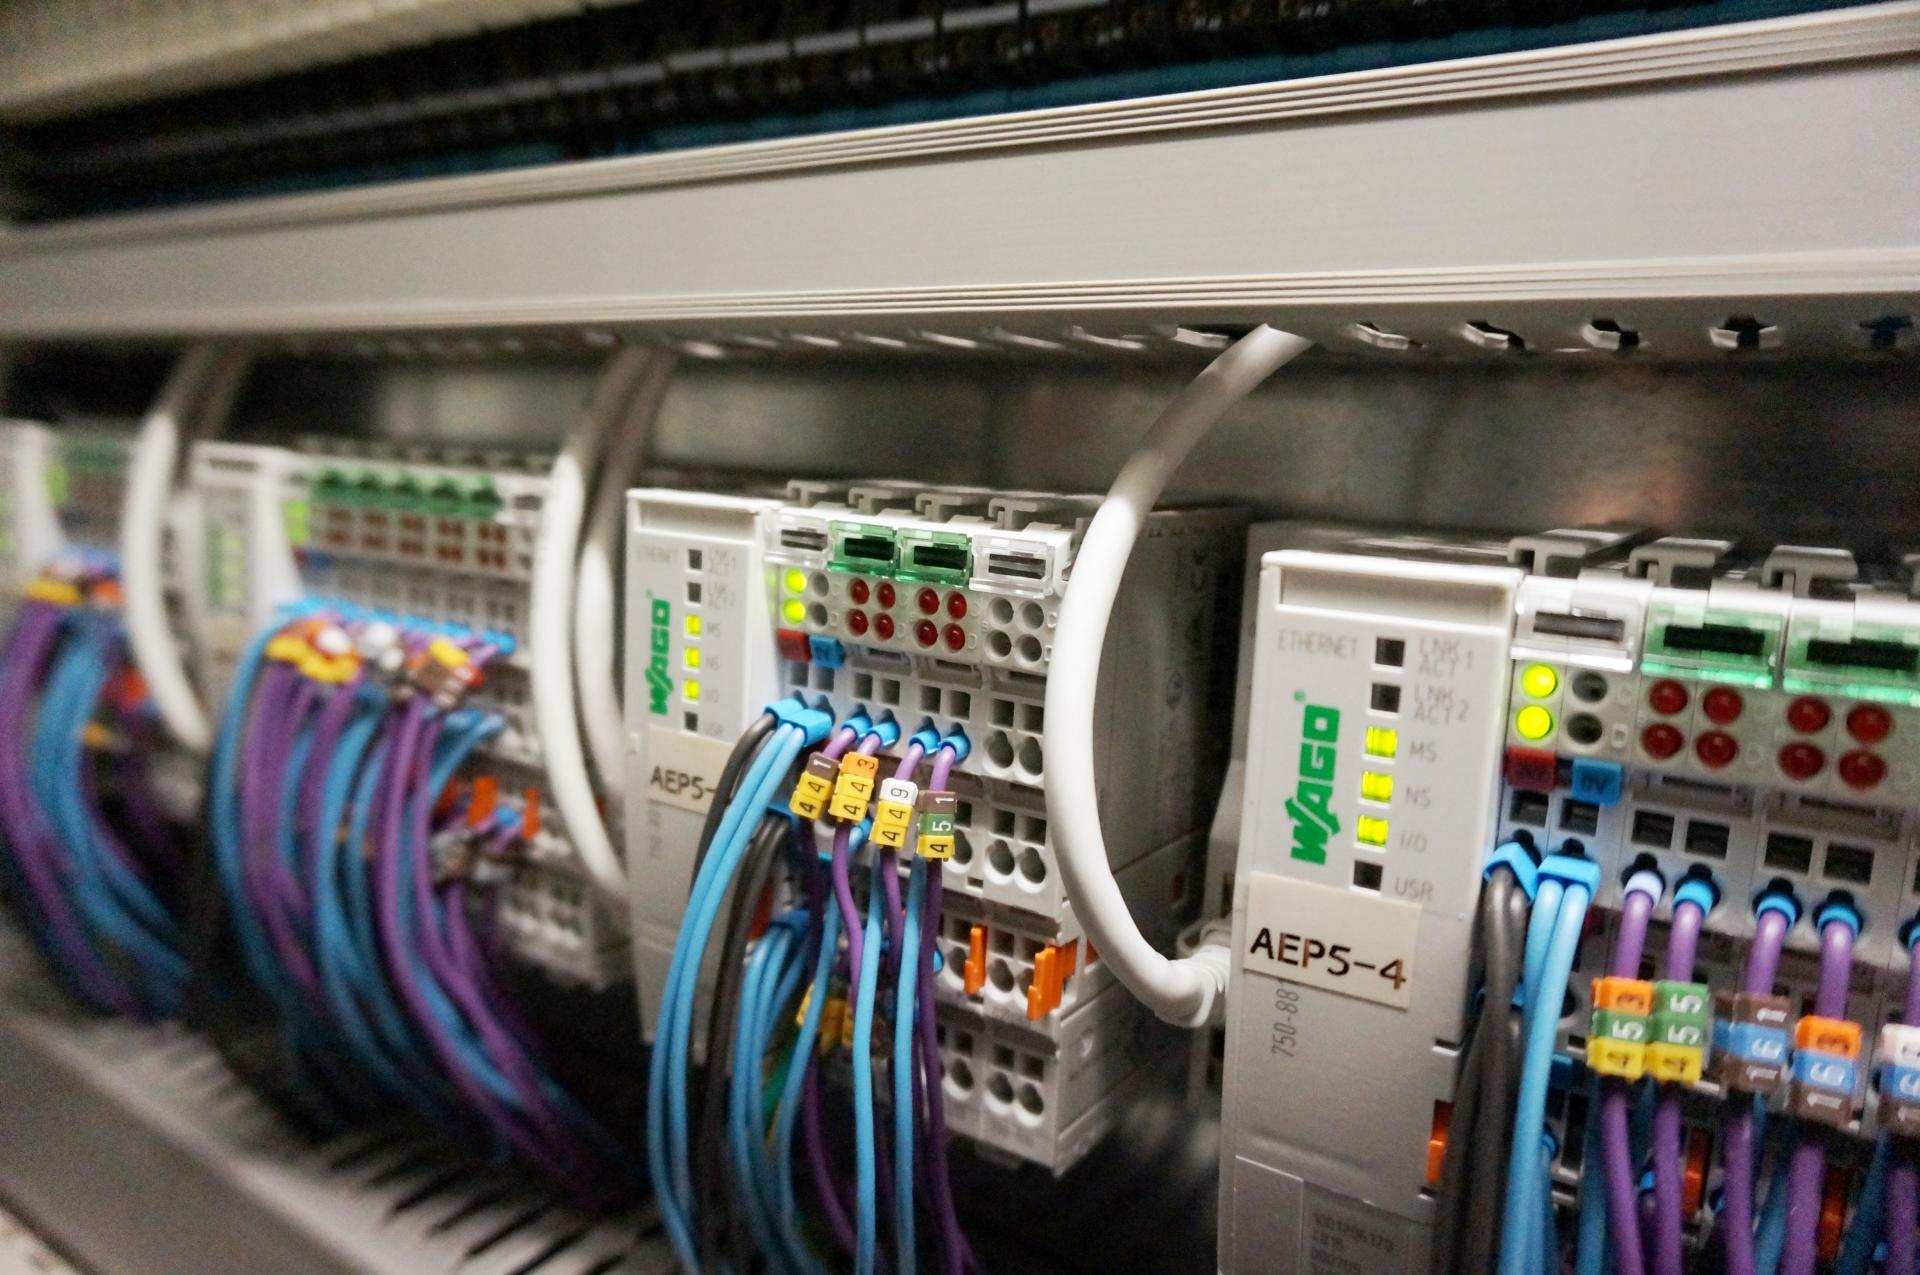
\includegraphics[width=\columnwidth]{data/plc.jpg}
		\caption{PLC modules.}
		\end{figure}
	\end{column}
\end{columns}
\end{frame}

%------------------------------------------------

\subsection{Model railways control}

\begin{frame}{Context: PLC in model railroads}
\begin{figure}
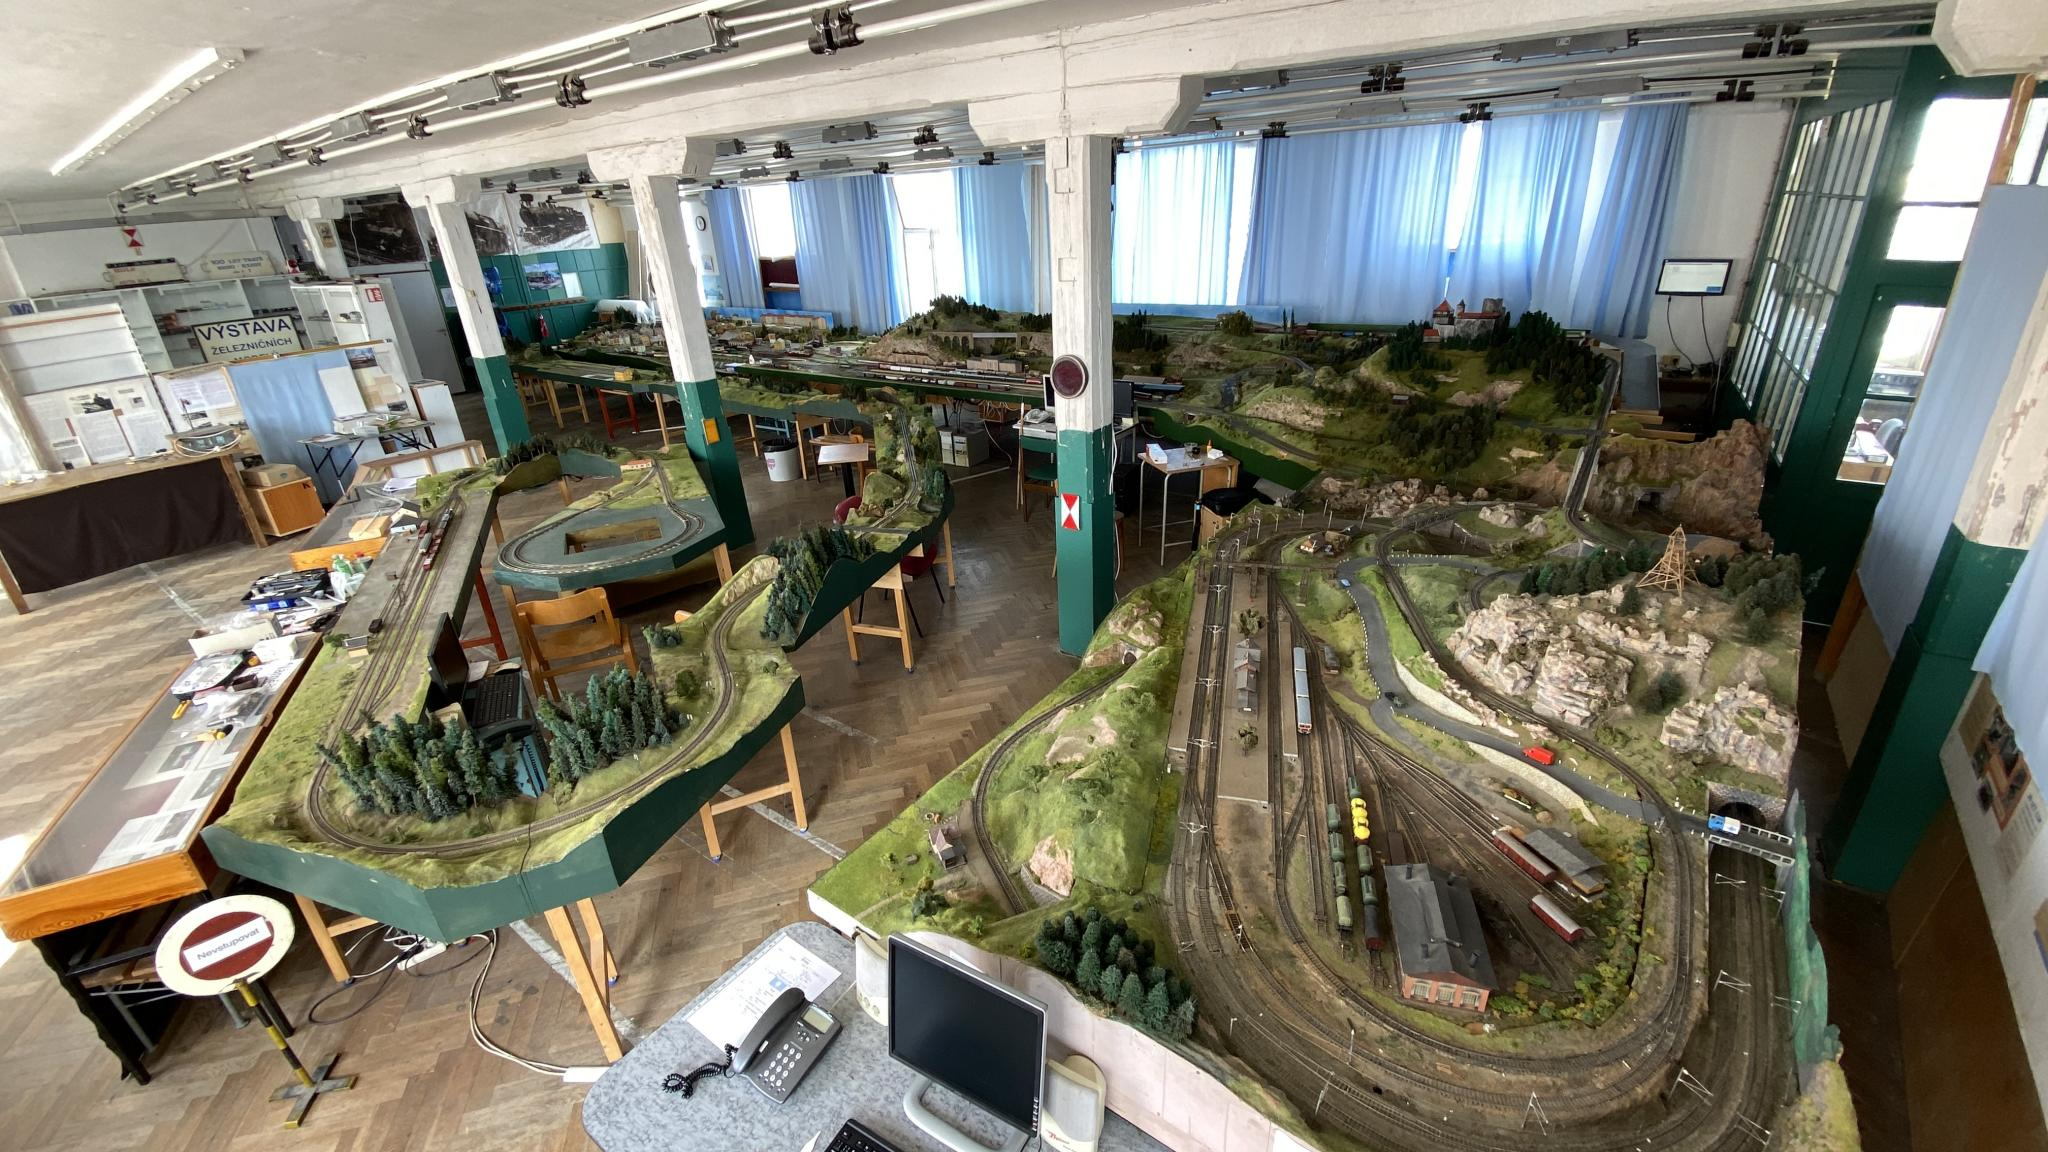
\includegraphics[width=0.8\columnwidth]{data/kolejisteMosilana.jpg}
\end{figure}
\end{frame}

%------------------------------------------------

\begin{frame}{Context: PLC in model railroads}
\begin{columns}
	\begin{column}{.3\textwidth}
		\begin{itemize}
		\item 13 stations.
		\item 186 switches.
		\item 306 track circuits.
		\item 233 signals.
		\item 13 crossings.
		\item 100 disconnectors.
		\item \textbf{70 MTB modules.}
		\end{itemize}
	\end{column}
	\begin{column}{.65\textwidth}
		\begin{figure}
		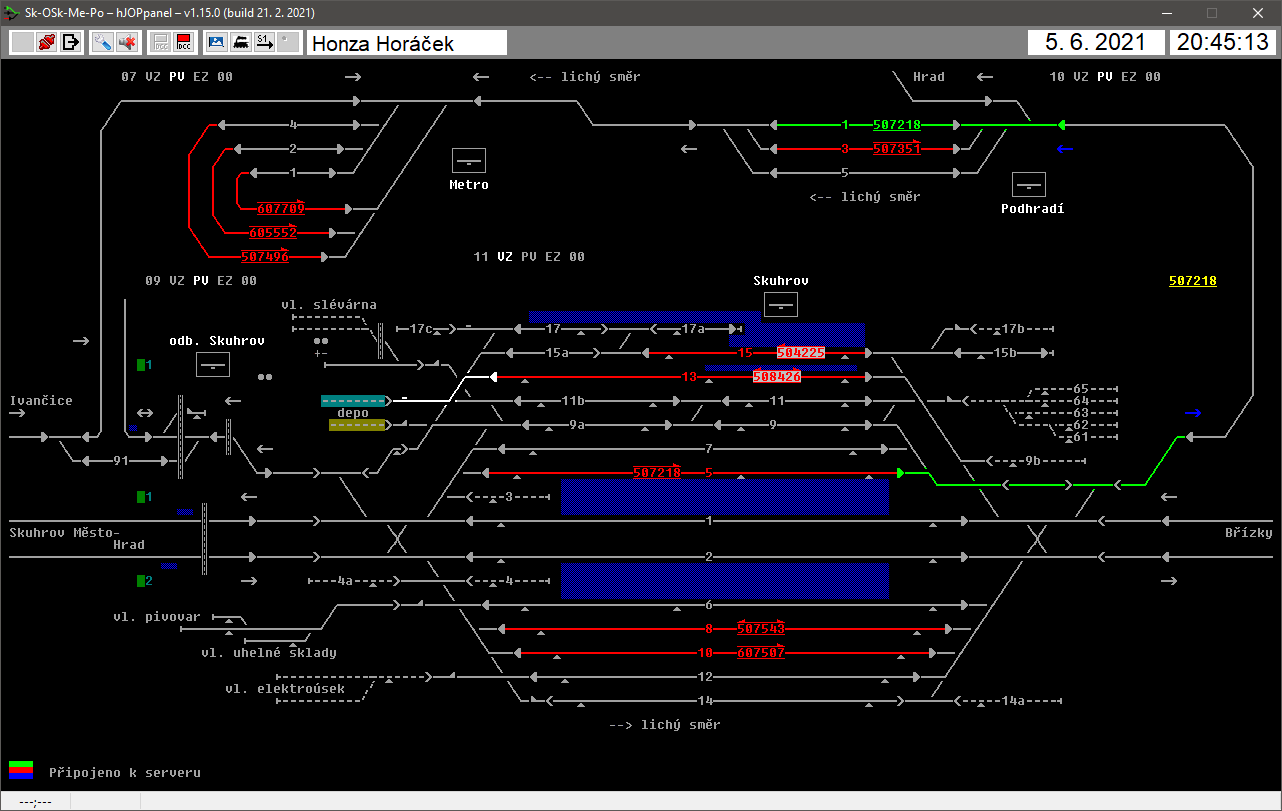
\includegraphics[width=\columnwidth]{data/sk.png}
		\caption{Model railway control software interface.}
		\end{figure}
	\end{column}
\end{columns}
\end{frame}

%------------------------------------------------

\begin{frame}{MTB \& current deployment}
\begin{columns}
	\begin{column}{.6\textwidth}
		\begin{itemize}
		\item Own system designed in $\sim$2000.
		\item 1 model railway = 1 MTBbus.
		\begin{itemize}
			\item 1 MTB-USB module, many \textit{MTB modules}.
		\end{itemize}
		\item \textit{Master-slave} topology.
		\item MTB module types:
		\begin{enumerate}
			\item MTB-UNI, MTB-UNIm,
			\item MTB-TTL,
			\item MTB-REG,
			\item MTB-POT.
		\end{enumerate}
		\item MTB is used for controlling \textit{accessories}, not track.
		\end{itemize}
	\end{column}
	\begin{column}{.4\textwidth}
		\begin{figure}
		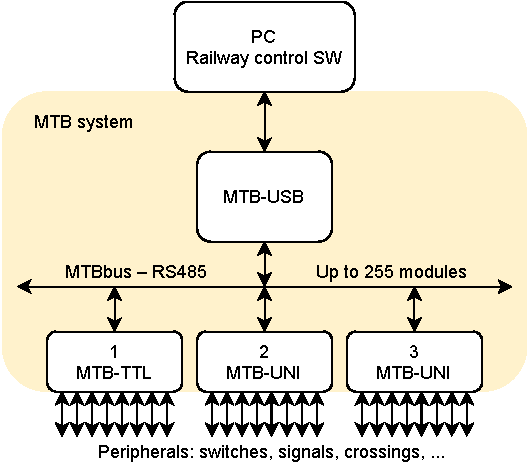
\includegraphics[width=\columnwidth]{data/mtb-topology-en.pdf}
		\caption{MTB v2 topology.}
		\end{figure}
	\end{column}
\end{columns}
\end{frame}

%------------------------------------------------

\subsection{MTBv4 design}

\begin{frame}{MTB v4 design}
\begin{columns}
	\begin{column}{.3\textwidth}
		New components designed:
		\begin{enumerate}
		\item MTBbus protocol,
		\item MTB-USB v4,
		\item MTB-UNI v4,
		\item MTB-2-AVR,
		\item IRdet,
		\item MTB Daemon,
		\item hJOP MTB RCS Network Library.
		\end{enumerate}
	\end{column}
	\begin{column}{.4\textwidth}
		\begin{figure}
		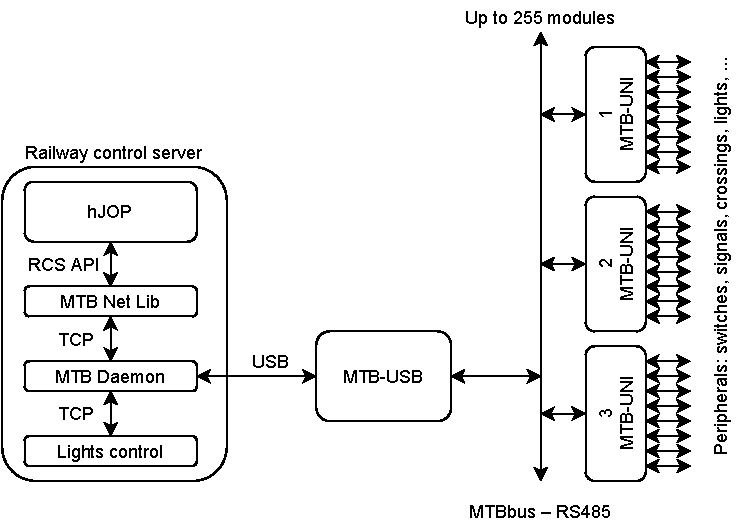
\includegraphics[width=\columnwidth]{data/new-topology-en.pdf}
		\caption{MTB v4 topology.}
		\end{figure}
	\end{column}
	\begin{column}{.3\textwidth}
		\begin{figure}
		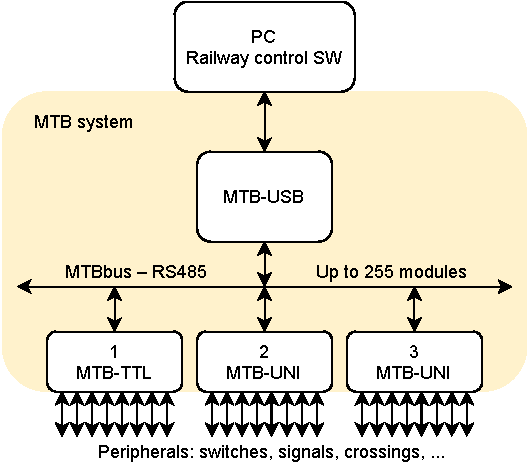
\includegraphics[width=\columnwidth]{data/mtb-topology-en.pdf}
		\caption{MTB v2 topology.}
		\end{figure}
	\end{column}
\end{columns}
\end{frame}

%------------------------------------------------

\subsection{MTBbus}

\begin{frame}{MTBbus v4}
\begin{columns}
	\begin{column}{.5\textwidth}
		\begin{itemize}
		\item Hardware layer kept: RS485.
		\item New protocol designed from scratch.
		\begin{itemize}
			\item Speed $38\ 400$ – $115\ 200$ Bd
			\item 9-bit communication.
			\item \textit{master-slave} principle.
		\end{itemize}
		\item Module must respond to each \textit{message}.
		\end{itemize}
	\end{column}
	\pause
	\begin{column}{.5\textwidth}\texttt{\footnotesize
> Module 1 Inquiry \\
< Acknowledgement  \# Modul 1 alive, \\
  no data to send \\
> Module 2 Inquiry \\
\# Timeout – module 2 down \\
> Module 3 Inquiry \\
< State of inputs changed, \\
  new state: 0b00001010 0b11110000 \\
> Module 6 Inquiry \\
< Acknowledgement \\
> Set Outputs of module 1 to\\
  0b00101010 0b01000101 \\
< Outputs Set to 0b00101010 0b01000101 \\
> Module 10 Inquiry \\
< Acknowledgement \\
...}
	\end{column}
\end{columns}
\end{frame}

%------------------------------------------------

\section{Nový hardware}
\subsection{MTB-USB v4}

\begin{frame}{MTB-USB v4}
\begin{columns}
	\begin{column}{.4\textwidth}
		\begin{figure}
		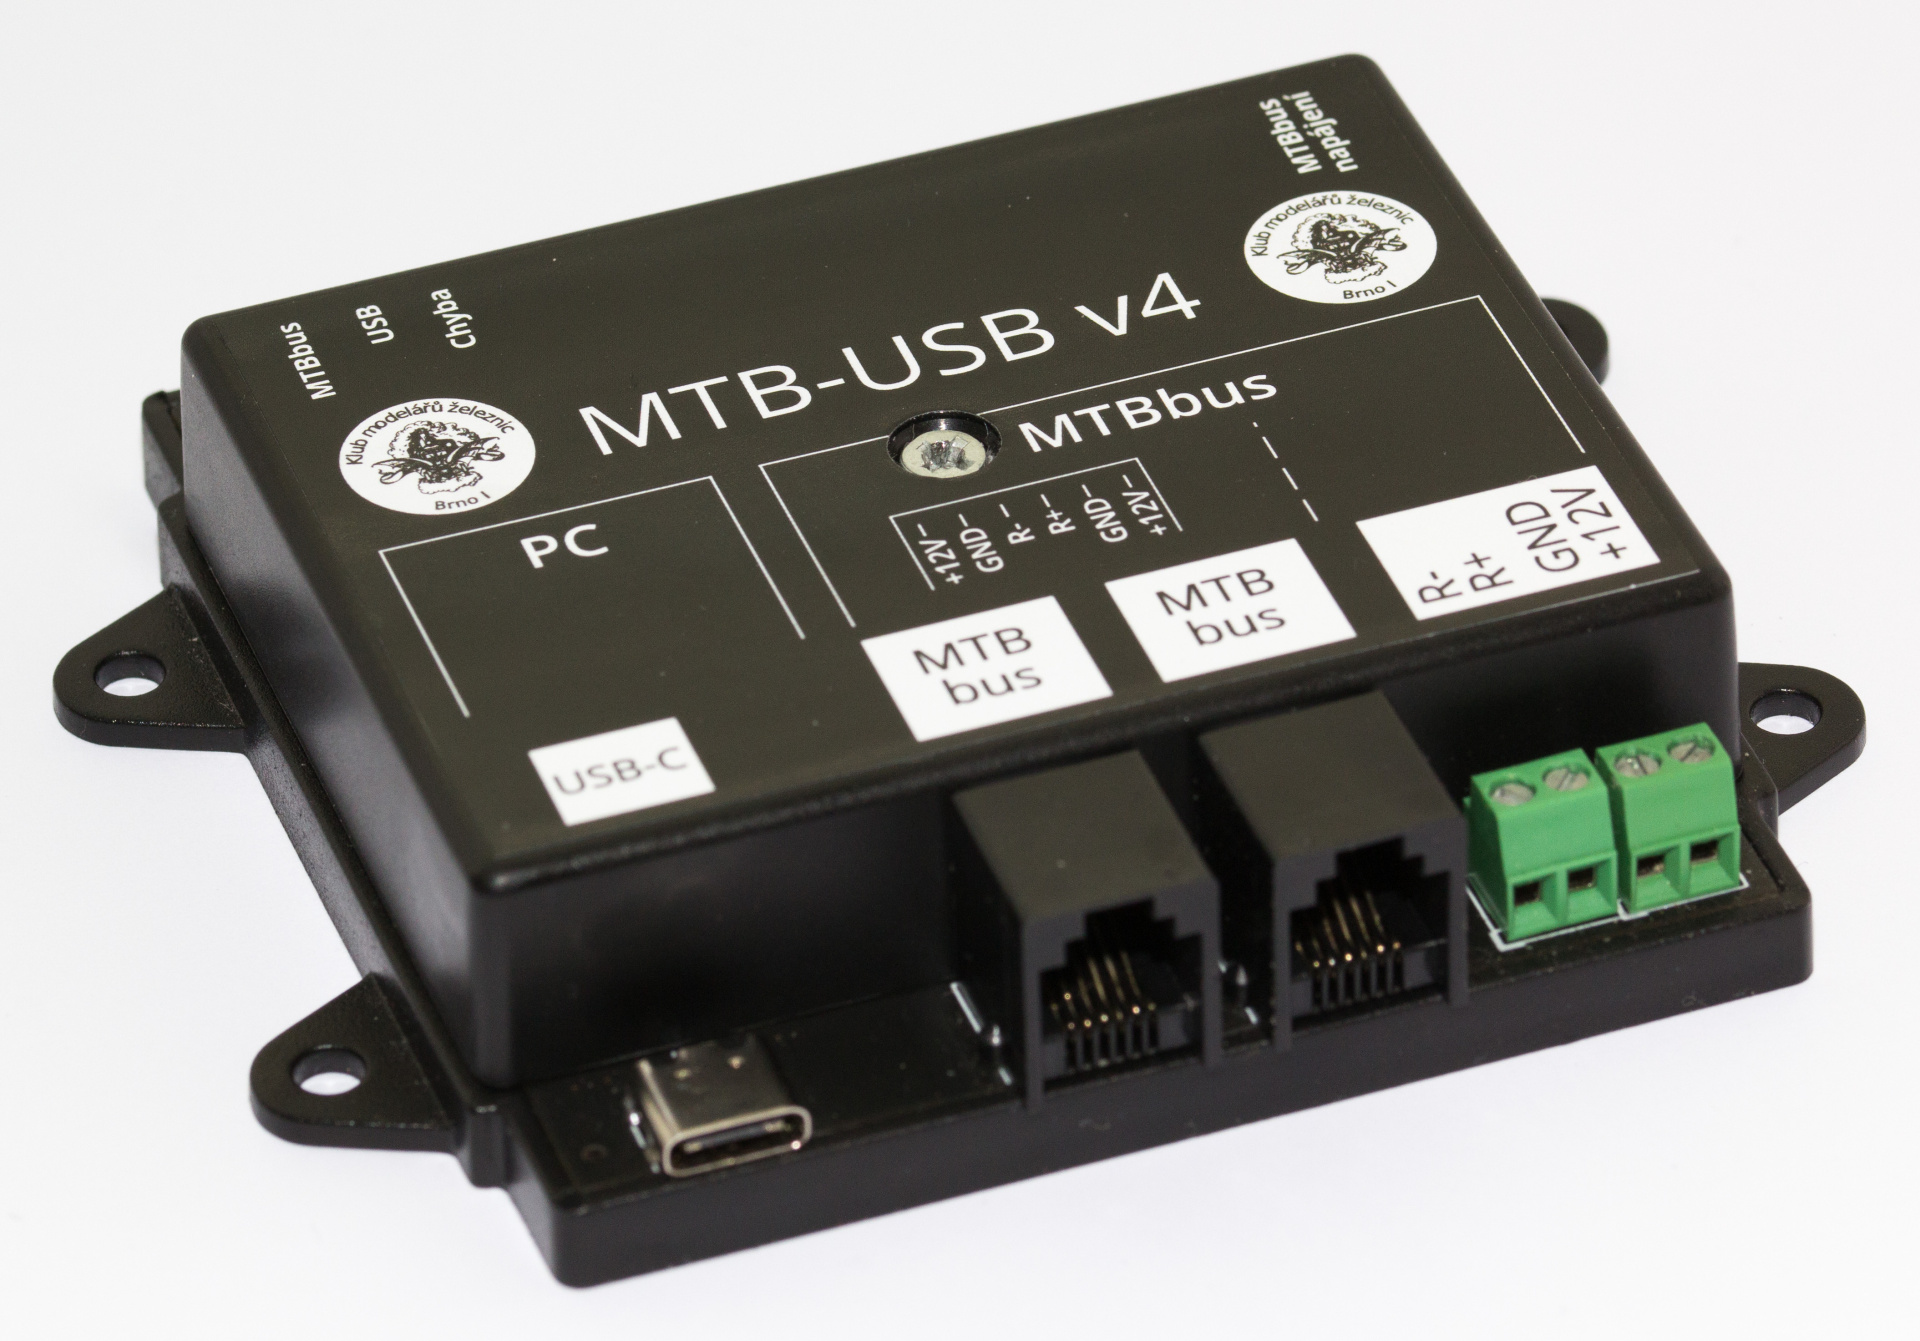
\includegraphics[width=\columnwidth]{data/usb-all.jpg}
		\end{figure}
	\end{column}
	\begin{column}{.6\textwidth}
		\begin{figure}
		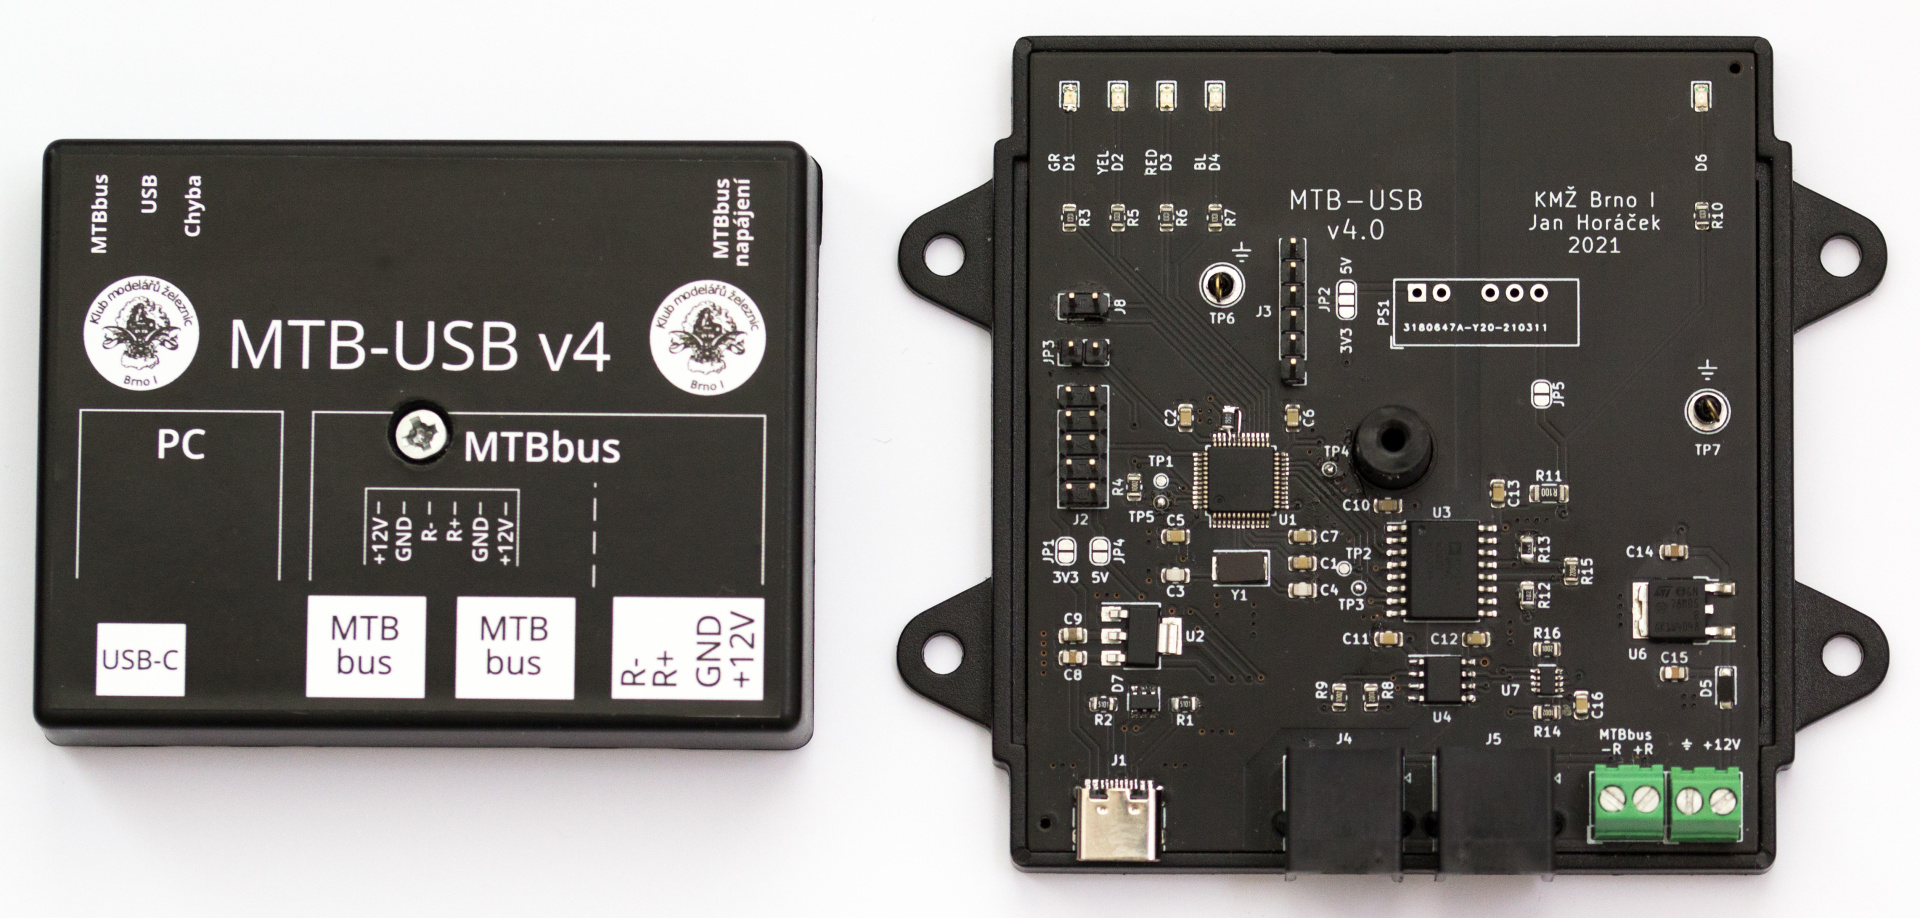
\includegraphics[width=\columnwidth]{data/usb-inside.jpg}
		\end{figure}
	\end{column}
\end{columns}
\end{frame}

%------------------------------------------------

\begin{frame}{MTB-USB v4}
\begin{enumerate}
\item Retransmits data between MTBbus \& PC.
\item Intentionally does not contains complicated logic.
\item Performs time-critical operations of MTBbus.
\item Performs modules \textit{polling}.
\item Maintains list of active modules.
\item Retransmits MTBbus data in case of delivery errors.
\end{enumerate}
\end{frame}

%------------------------------------------------

\begin{frame}{Hardware}
\begin{itemize}
\item Galvanically separated USB \& MTBbus parts on PCB.
\begin{itemize}
\item USB part powered via USB-C.
\item MTBbus part powered via DC-DC converter or externally.
\end{itemize}
\item Processor \texttt{STM32F103}.
\begin{itemize}
\item Direct USB support.
\item USB part of PCB.
\end{itemize}
\item RS485 driver \texttt{ADM2483}.
\item Automatic SMT on \textit{JLCPCB}.
\item KiCad.
\end{itemize}
\end{frame}

%------------------------------------------------

\begin{frame}{Firmware}
\begin{itemize}
\item C
\item STM32 HAL
\item DMA
\item $\sim$2700 LOC
\end{itemize}
\end{frame}

%------------------------------------------------

\subsection{MTB-UNI v4}

\begin{frame}{MTB-UNI v4}
\begin{columns}
	\begin{column}{.5\textwidth}
		\begin{itemize}
		\item 16 digital inputs.
		\item 16 digital outputs.
		\item Power: 7–17 V DC.
		\item Addressing via jumpers.
		\item Processor ATmega128.
		\begin{itemize}
			\item Main program + bootloader.
			\item C
			\item $\sim$1600 LOC
		\end{itemize}
		\item Eagle.
		\end{itemize}
	\end{column}
	\begin{column}{.5\textwidth}
		\begin{figure}
		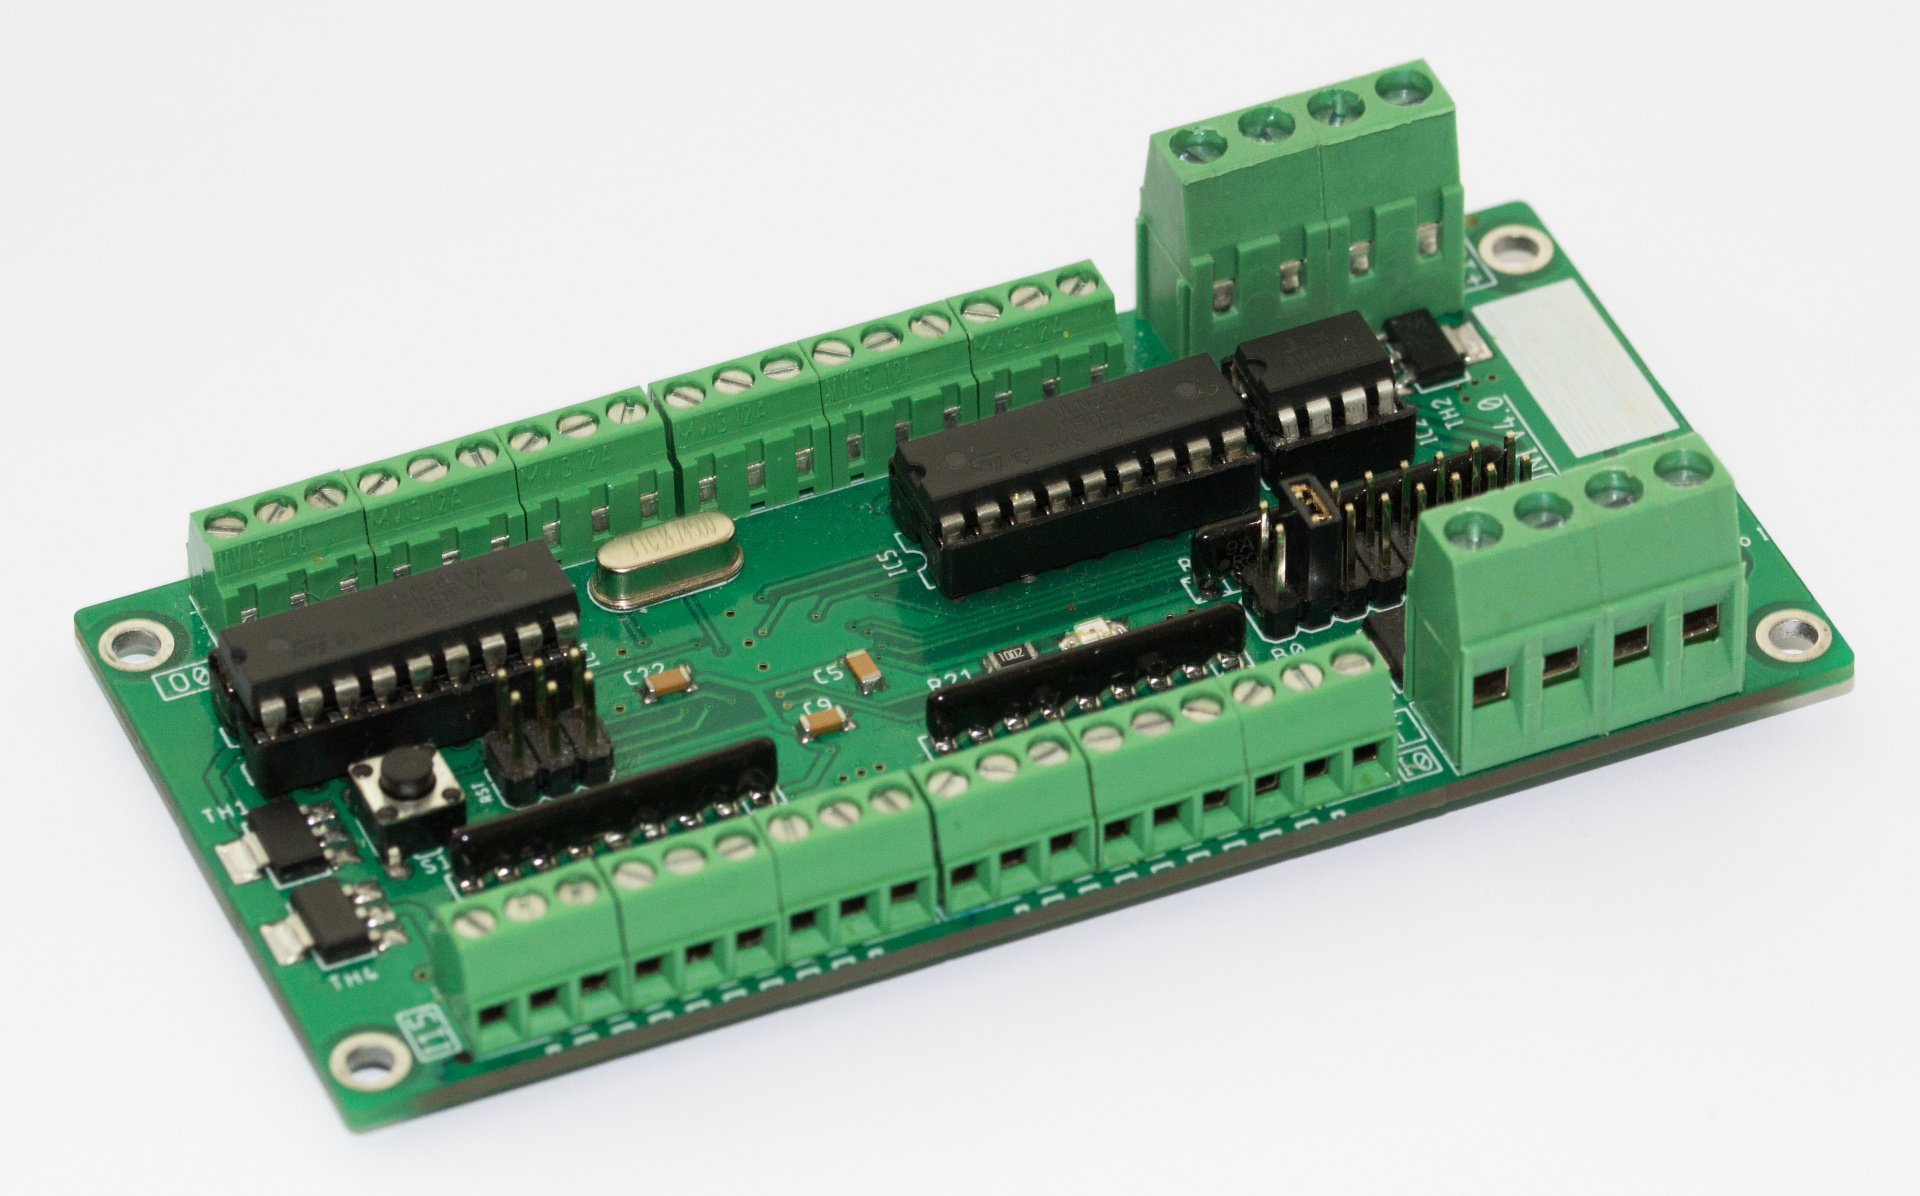
\includegraphics[width=\columnwidth]{data/uni-v40-screw-all.jpg}
		\caption{MTB-UNI v4 module.}
		\end{figure}
	\end{column}
\end{columns}
\end{frame}

%------------------------------------------------

\subsection{MTB-2-AVR}

\begin{frame}{MTB-2-AVR}
\begin{columns}
	\begin{column}{.5\textwidth}
		\begin{itemize}
		\item PCB replaces CPU in old MTB modules.
		\item Universal PCB for all old MTB modules.
		\item Upgrade to MTBbus v4 does not require all modules to be replaced.
		\item Processor ATmega328p.
		\begin{itemize}
			\item Main program + bootloader.
			\item C
			\item 2100 LOC
		\end{itemize}
		\item Eagle.
		\end{itemize}
	\end{column}
	\begin{column}{.5\textwidth}
		\begin{figure}
		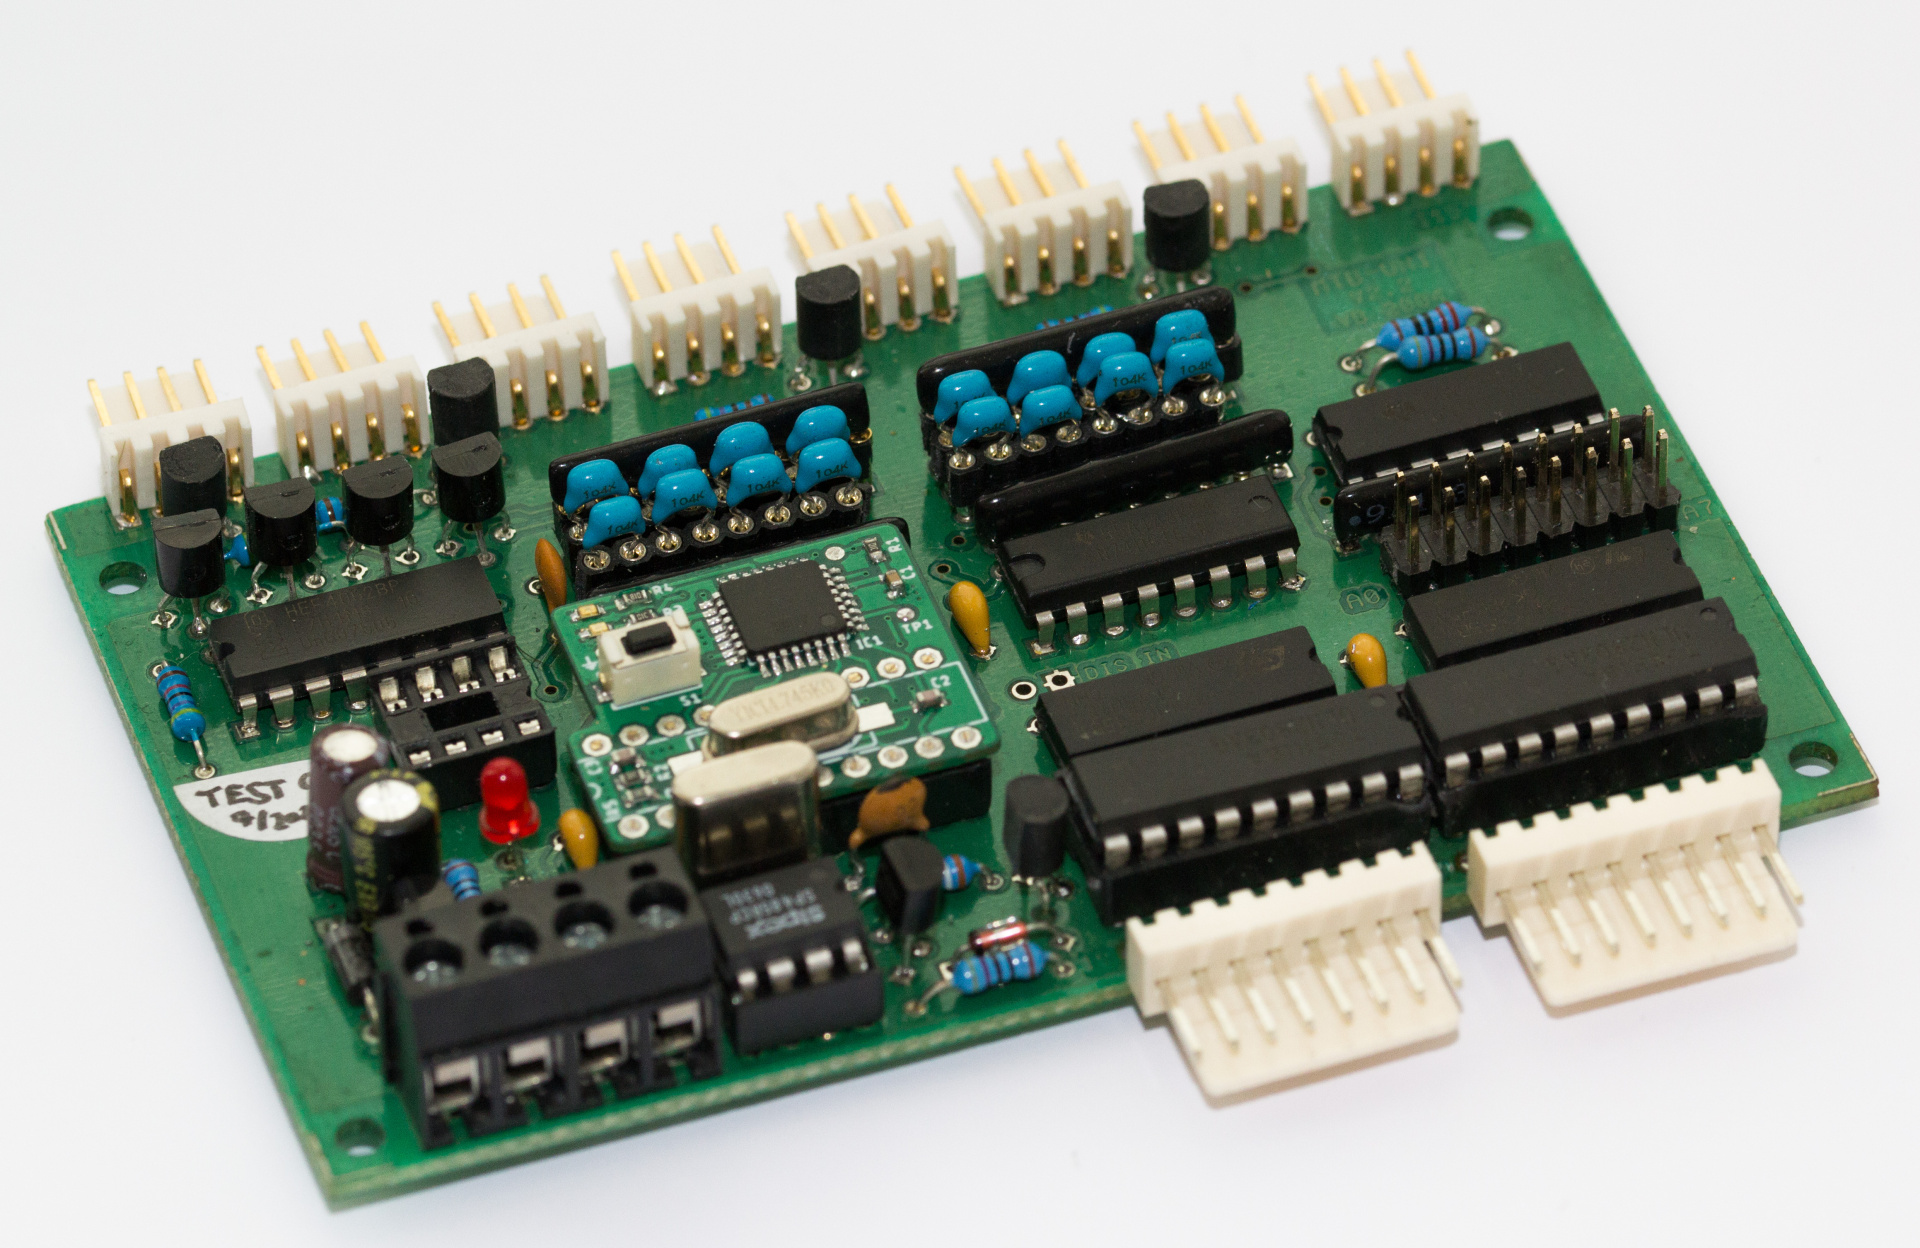
\includegraphics[width=\columnwidth]{data/uni-2-upgrade-all.jpg}
		\caption{MTB-2-AVR PCB in old MTB-UNI v2 module.}
		\end{figure}
	\end{column}
\end{columns}
\end{frame}

%------------------------------------------------

\subsection{IRdet}

\begin{frame}{IRdet}
\begin{columns}
	\begin{column}{.7\textwidth}
		\begin{itemize}
		\item Replaces direct support of IR inputs in MTB-UNI v2.
		\item Not connected to MTBbus.
		\item 8 IR inputs.
		\item 8 digital optically separated outputs.
		\item Universal.
		\item Eagle.
		\end{itemize}
	\end{column}
	\begin{column}{.3\textwidth}
		\begin{figure}
		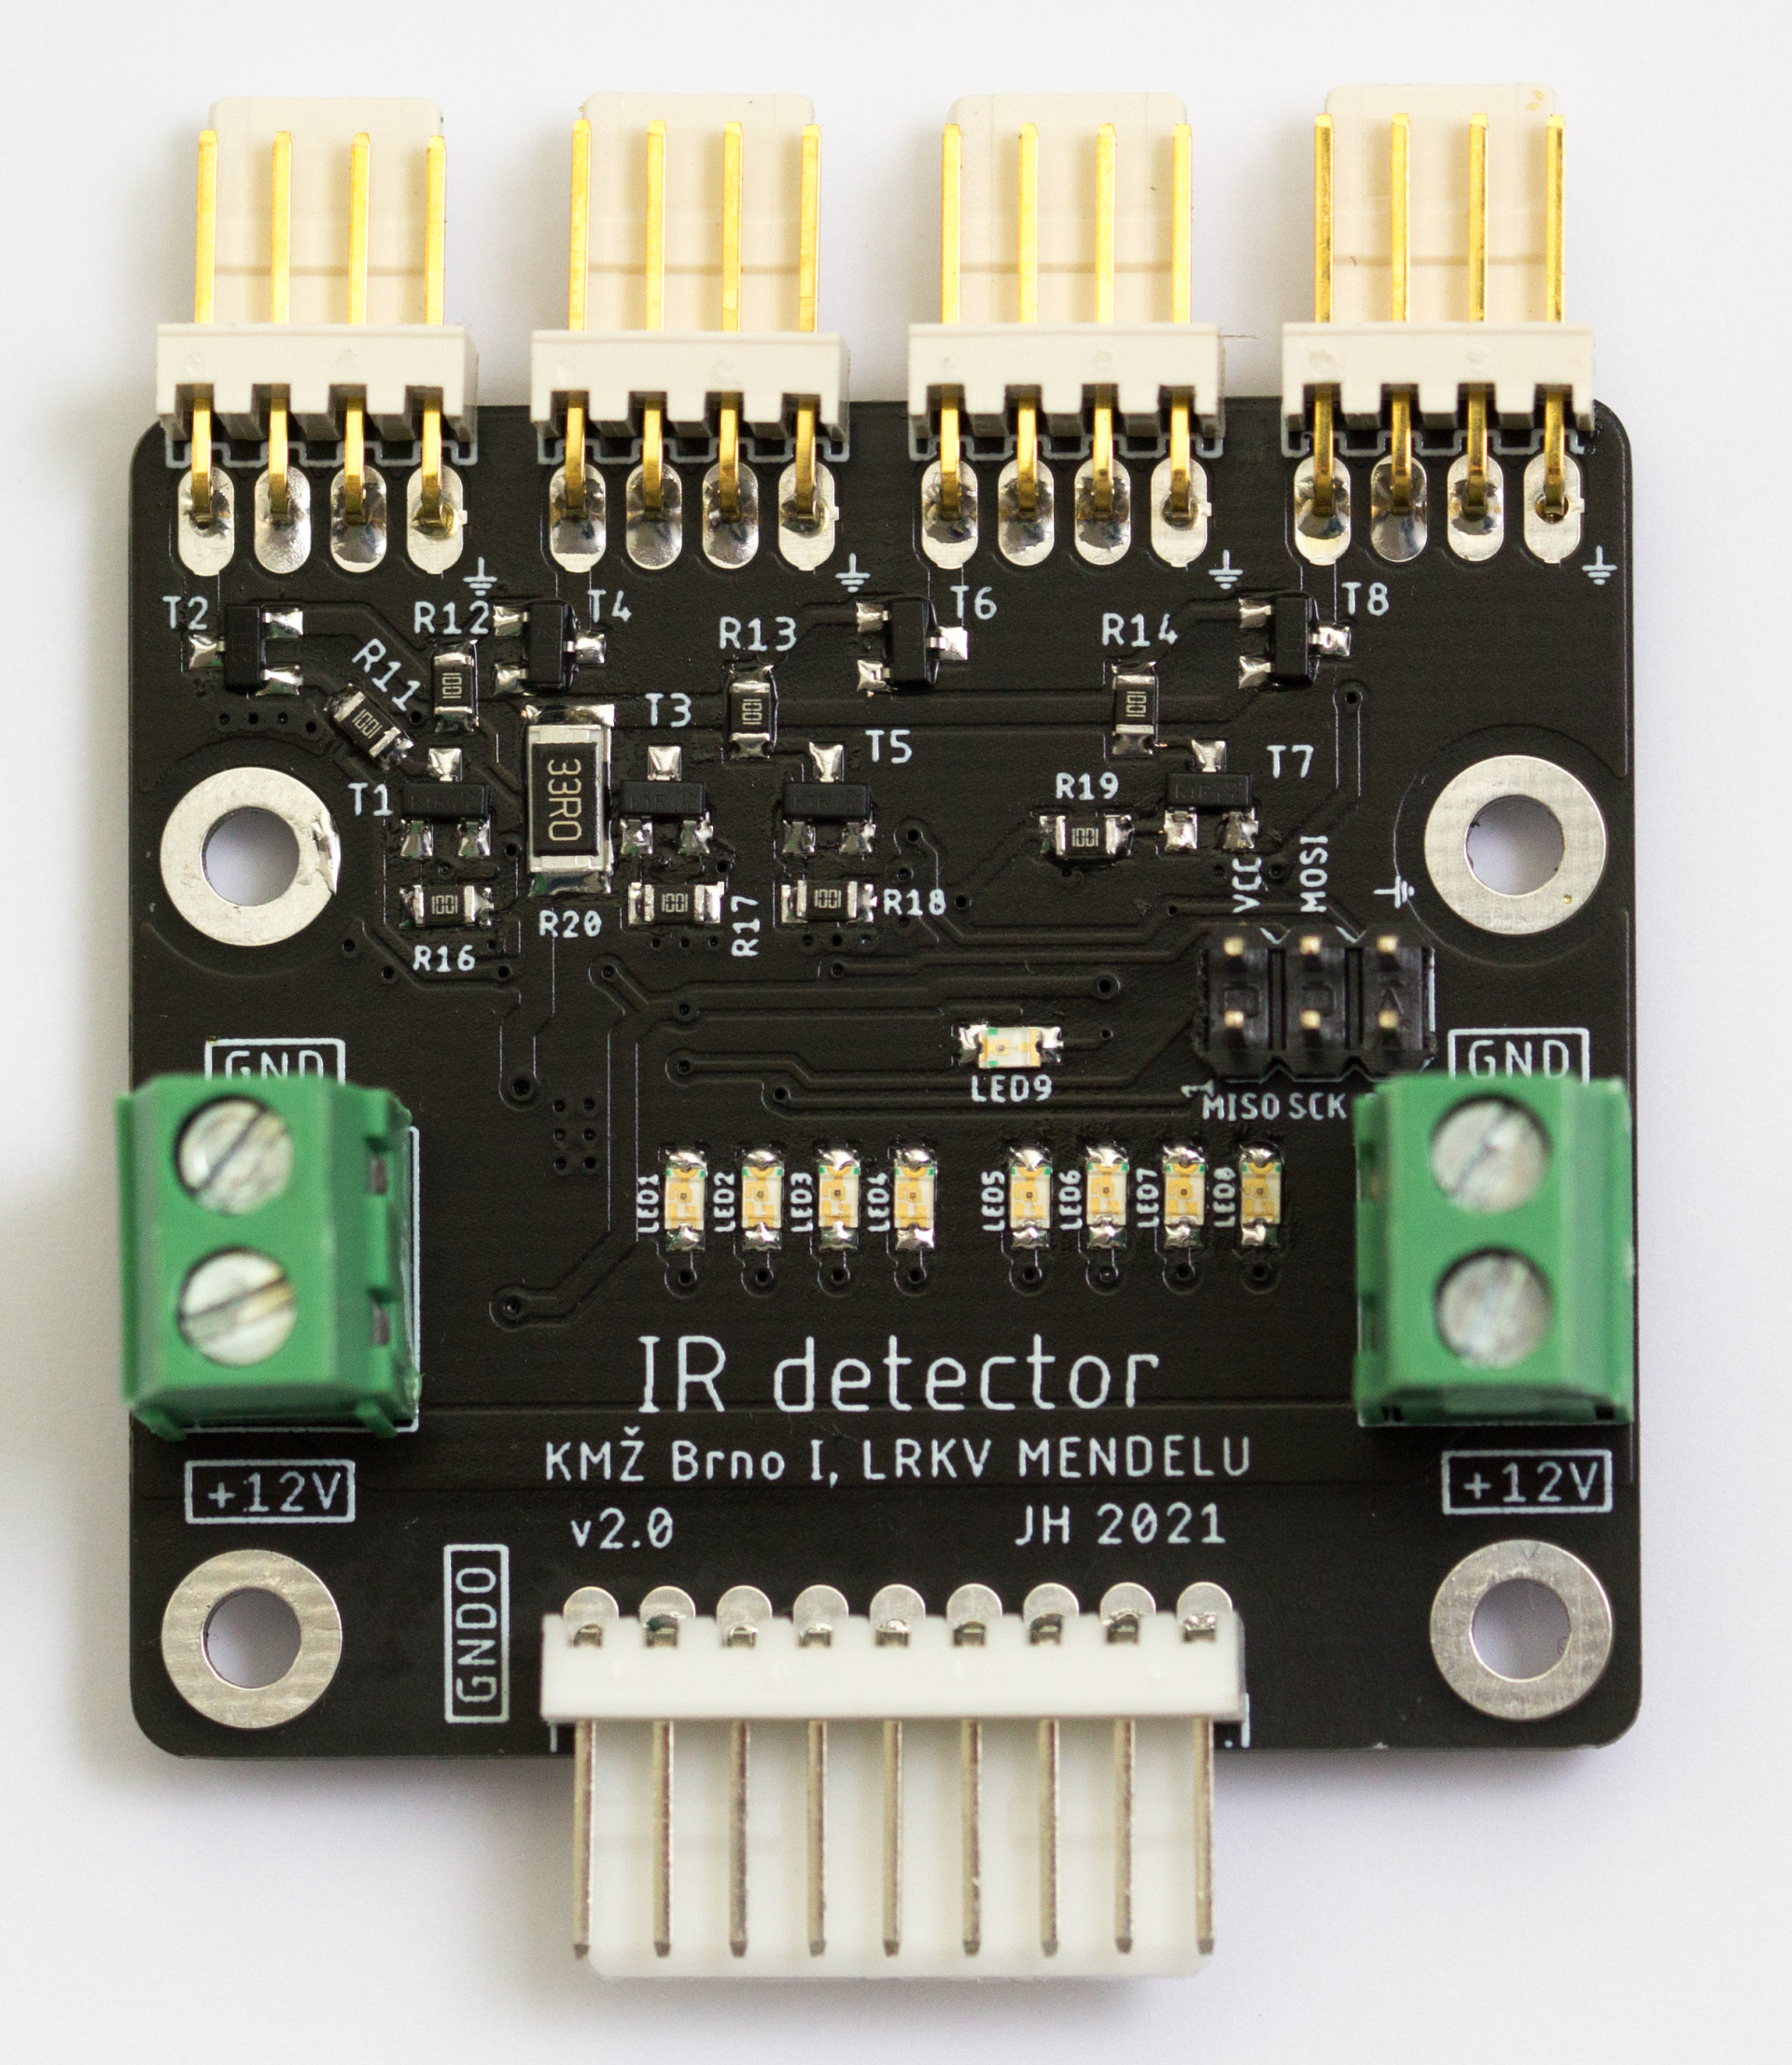
\includegraphics[width=\columnwidth]{data/irdet-front.jpg}
		\caption{IRdet PCB.}
		\end{figure}
	\end{column}
\end{columns}
\end{frame}

%------------------------------------------------

\section{Conclusion}

\begin{frame}{Components designed}
\begin{columns}
	\begin{column}{.5\textwidth}
		\begin{enumerate}
		\item MTBbus protocol,
		\item MTB-USB v4,
		\item MTB-UNI v4,
		\item MTB-2-AVR,
		\item IRdet,
		\item MTB Daemon,
		\item hJOP MTB RCS Network Library.
		\end{enumerate}
	\end{column}
	\begin{column}{.5\textwidth}
		\begin{figure}
		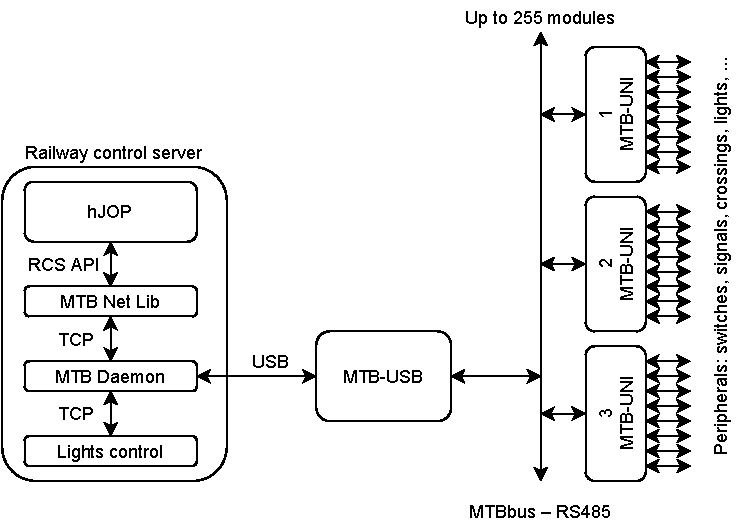
\includegraphics[width=\columnwidth]{data/new-topology-en.pdf}
		\caption{Topology of MTB v4.}
		\end{figure}
	\end{column}
\end{columns}
\end{frame}

%------------------------------------------------

%\section{\bibname}
%\begin{frame}[t, allowframebreaks]{\bibname}
%\printbibliography[heading=none]
%\end{frame}

%------------------------------------------------

\end{document}
